\chapter{Related software}

There are plenty of programs and libraries for \gls{graph} visualization with different purposes.
Just to name a few there are D3.js, Neo4j, Graphviz, Tulip, Wolfram Grapher, Pajek and many more.

In this chapter however I'm going to focus on just three software products - each with very different use-case and target userbase.

\begin{itemize}

\item The first one is \textbf{Obsidian} which is primarily a note-taking application
but provides a graph view of the notes as an interesting and easy to use feature. 

\item The second is \textbf{Gephi}, a software focused on in-depth analysis and visualization of large graphs.

\item And finally there's \textbf{Cytoscape.js}. A javascript library for graph visualization in the browser.

\end{itemize}

We chose these in particular because Aphantasia could be viewed as a hybrid of the trio.

We will look into three aspects of these products:
\begin{itemize}
  \item Primary use-case and target userbase
  \item User experience
  \item Ability to visualize large graphs
\end{itemize}

As the source of data for testing the large-graph visualization capabilities we chose the dataset of citations between papers
in the field of high-energy physics \cite{snap_cit_hep} (Later refered to as \gls{cithep_dataset}).
It contains 34546 nodes, 421578 edges and temporal data.

This dataset is suitable for our purposes because:
\begin{itemize}
  \item It's large enough to test the the capabilities of both the mentioned software and Aphantasia
  \item It's a real-world dataset with temporal data which is going to play a role in visualizing the contents of Aphantasia
\end{itemize}

\section{Obsidian}

Obsidian \cite{obsidian_website} was a direct inspiration for Aphantasia. It allows users to create, edit and most importantly interlink markdown file notes in the file system.
One Obsidian project is just a system directory called a Vault. It is a set of markdown notes, user settings, plugins and other files.
The interlinked notes in a Vault form a directed graph which can be visualized with just a click of a button.
The graph is animated and has the ability to replay the history of the Vault from the very first note to the current state.

It's clear from this description that Obsidian is aimed at general audience of note-takers 
with maybe a slight bias towards graph/data visualization enthisuiasts.
It's available for all the major operating systems and has a large community of users and plethera of extensions available through the
community plugins.

\subsection*{Obsidian graph view}

The graph visualization in obsidian (called graph view) is easy to use and provides an appealing visual representation of the notes.
The graph is animated and interactive, meaning that the user can drag nodes around, zoom in and out and click on nodes to open the associated note.

It is also customizable to some extent.
Colors of the nodes can be set based on different filters such as path, tags or text-search.
Users can also adjust four sliders - central force, repel force, link force and link distance.
The graph view is sufficient for small graphs but for larger graphs the program needs to spend some time indexing the notes.
(Though, this is a one-time operation and the indexes are then saved in the Vault).

In figure \ref{obr:obsidian_common} you can see a typical Obsidian graph view depicting a small Vault of one of our personal projects.

In figure \ref{obr:obsidian_3000} we converted a part of the CitHep dataset with only the first 3000 nodes
\footnote{The first as in the order they are stored in the dataset file.}
to markdown notes and visualized it in Obsidian.
It took our machine over 10 minutes to index this graph.
Once indexed however the application ran smoothly.

We were unable to visualize the whole dataset without the program crashing or taking too long to index.
We did however find several examples of larger datasets rendered in Obsidian online
\cite{obsidian_reddit_large_graph}.

Obsidian is not very good at clustering nodes with high degree of connectivity.
To our knowledge it also has no support for automatic colouring of the nodes based on clusters, modularity  or other data indicators.
Color has to be user defined based on content and location of the notes.
CitHep nodes do not contain any content apart from id and date which is why the graph in figure \ref{obr:obsidian_3000} is all default gray.

\begin{figure}[p]\centering
  \includegraphics[width=140mm, keepaspectratio]{img/obsidian_common_notes.png}
  \caption{A common graph view of a small Vault in Obsidian}
  \label{obr:obsidian_common}
\end{figure}


\begin{figure}[p]\centering
  \includegraphics[width=140mm, keepaspectratio]{img/Obsidian_3000}
  \caption{The first 3000 nodes of the CitHep dataset visualized in Obsidian}
  \label{obr:obsidian_3000}
\end{figure}

\section{Gephi}

Much more specialized than Obsidian, Gephi \cite{gephi_homepage} is an open source software focused on visualization and quantitative analysis of large graphs.
It provides several algorithms for graph layout and quantitative analysis of various data and is extendable through community plugins.

Gephi can compute quantitative characteristics of graph-based data such as modularity, clustering coefficient, degree distribution and many more.
It can not just vizualize the working data in the viewport but also export rather visually appealing images of the vizualized graph.

\subsection*{Gephi graph export}

In figure \ref{obr:gephi_cithep_3k} you can see, again, the first 3000 nodes of the CitHep dataset visualized in Gephi.
Compared with Obsidian the Gephi render export provides more visually identifiable characteristics of the data:

\begin{itemize}
  \item The layout is more structured and communities are more visible
  \item Colors of the nodes represent their associated modularity class
  \item Size of the nodes represents the number of citations the associated paper has
\end{itemize}

Figure \ref{obr:gephi_cithep} is an exported image of the entire CitHep dataset visualized in Gephi.
The process of exporting this image took a few hours.
We had to learn to use the program itself, import the data,
tweak the layout using various provided algorithms (though we mostly relied on ForceAtlas 2) and finally we exported the resulting image.

The software crashed a few times during the process and with the citHep dataset loaded in memory wasn't always buttery smooth but it was otherwise very usable.
Considering the amount of data that's a commendable feat.

Again, you can find even larger datasets visualized using Gephi.
One post on Gephi forum \cite{gephi_big_graph_forum} shows exported image made of 212 600 nodes and 4 045 203 edges.

The user experience of Gephi is one of a technical tool - something you have to learn to use and spend time with to get the most out of.
But the reward is the ability to visualize and analyze large graphs better than with any other software we could find.

\begin{figure}[p]\centering
  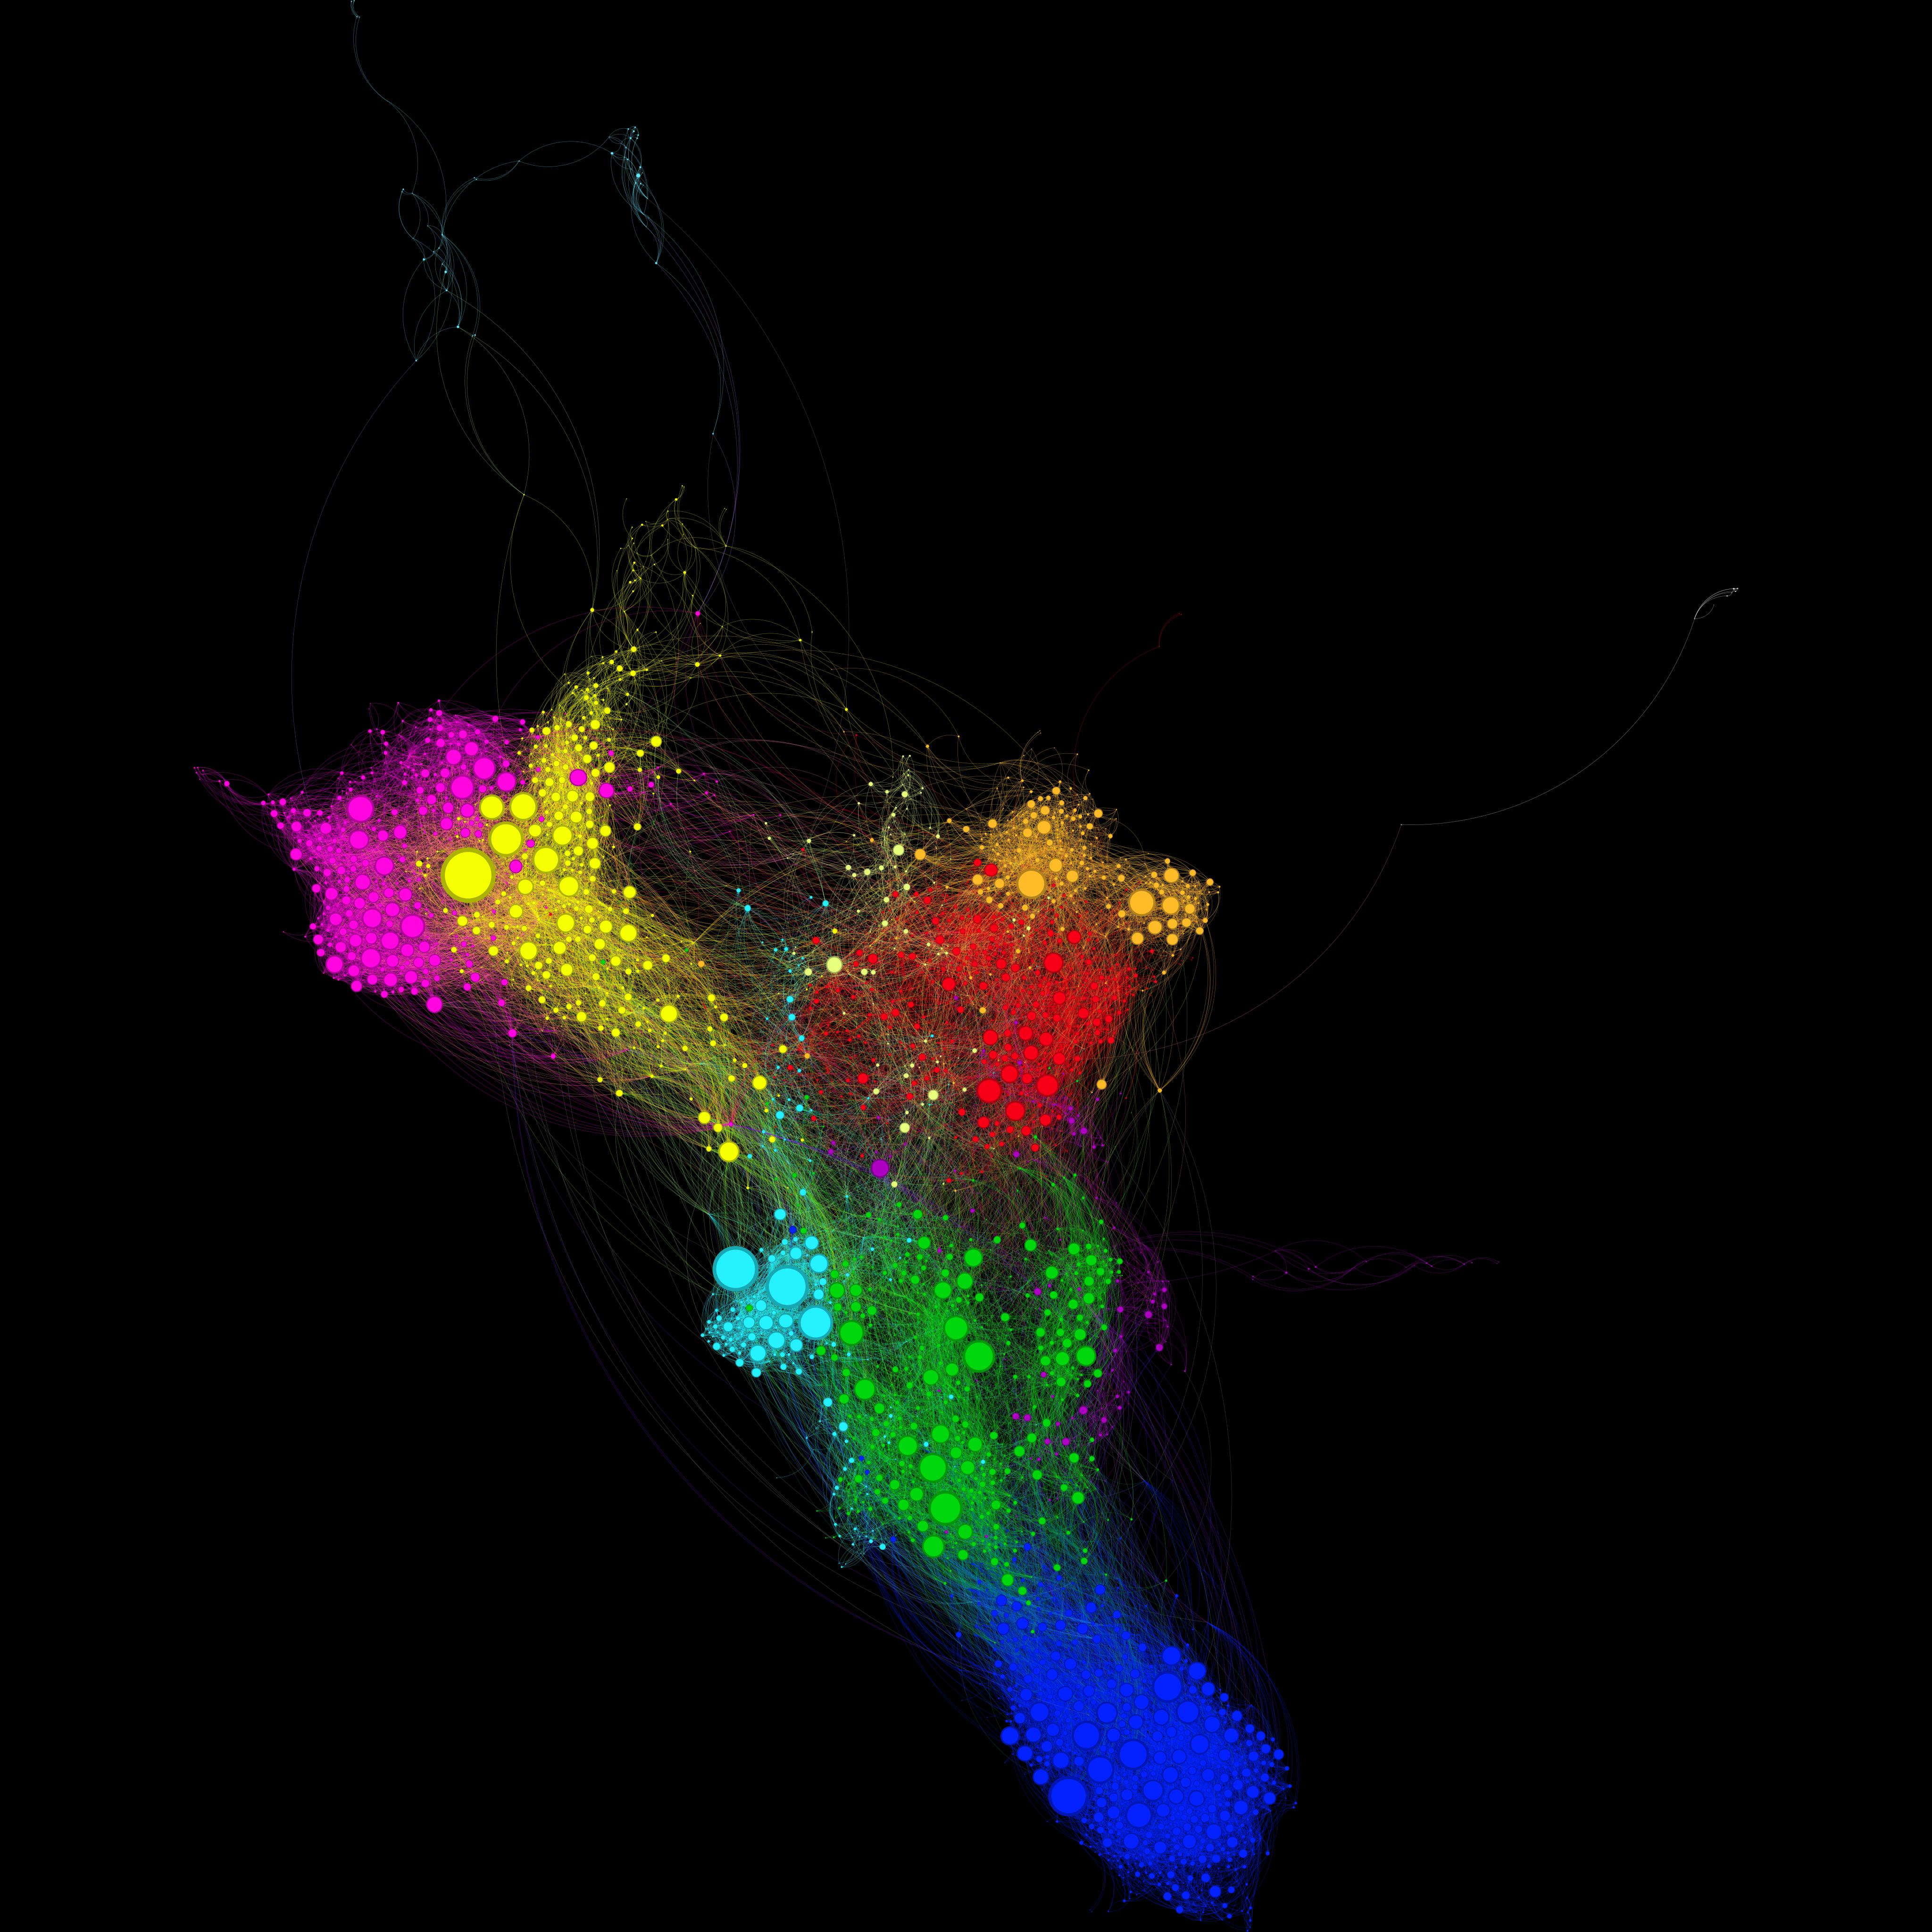
\includegraphics[width=140mm, keepaspectratio]{img/gephi_first_3000.png}
  \caption{The first 3000 nodes of the CitHep dataset visualized in Gephi}
  \label{obr:gephi_cithep_3k}
\end{figure}


\begin{figure}[p]\centering
  \includegraphics[width=140mm, keepaspectratio]{img/gephi_cithep_35k.png}
  \caption{CitHep dataset visualized in Gephi (34546 nodes)}
  \label{obr:gephi_cithep}
\end{figure}

\section{Cytoscape.js}

Cytoscape.js is a javascript library for graph visualization in the browser.
Its homepage starts with Demos section followed by headline 'Introduction' and almost 8200 lines of text \cite{cytoscapes_js_homepage}.
Among the demos there are various examples of usage ranging from simple \glspl{FDL} to more complex use-cases such as an interactive graph of wine and cheese pairings.
\cite{wine_and_cheese}

To assess the software we used two projects - a simple project of our own and one official template showcasing \gls{FDL} features of the library.

Firstly we attempted to create a react + cytroscpe.js project.
We initialized a fresh react ts project using \gls{vite}, added the dependency to cytoscpape and using the official instructions on the Cytoscape.js homepage we
created a simple application capable of rendering a graph.
See the result in figure \ref{obr:cytoscape_react_test}.
There is nothing particulary noteworthy about this attempt apart from the fact the the web application uses cytoscpe.js alongside react typescript
and seems to be a valid combination of libraries.


\begin{figure}[p]\centering
  \includegraphics[width=140mm, keepaspectratio]{img/cytoscape_react_10_nodes_path.png}
  \caption{A simple application in react + cytoscape rendering a simple graph}
  \label{obr:cytoscape_react_test}
\end{figure}

The second project was an attempt to render the CitHep dataset in Cytoscape.js.
In order to do so we cloned github repository of one of the official examples from the cytoscape.js homepage \cite{cytoscapes_js_github}.
The example is called 'Euler' and showcases several small demos using a cytoscape proprietary \gls{FDL}.

The demo called 'Large graph' showcases path of 5000 nodes and you can look the result in figure \ref{obr:cytoscape_5000_nodes_path}.

\begin{figure}[p]\centering
  \includegraphics[width=140mm, keepaspectratio]{img/cytoscape_5000_path_official_demo.png}
  \caption{An official example of large graph rendering in Cytoscape.js (path of 5000 nodes)}
  \label{obr:cytoscape_5000_nodes_path}
\end{figure}

This example is animated and on page refresh the graph stabilizes in real time.
We had to increase the simulation time as the default value resulted in a tangled unhelpful layout.
In this case the animation was realtively smooth and with the simulation time set to 10 seconds the graph layout worked well.

We modified this project to use, again, the first 3000 nodes from the CitHep dataset.
We tweaked several parameters such as force strength, edge length and repulsion strength and in the end we achieved layout shown in figure \ref{obr:cytoscape_3000_nodes}.
The performance during the runtime of the \gls{FDL} data dropped under 10 \gls{fps} but the application remained usable and stable.
The produced layout was very similar to the one we made with Obsidian.

\begin{figure}[p]\centering
  \includegraphics[width=140mm, keepaspectratio]{img/cytoscapejs_cithep_first_3000_nodes.png}
  \caption{The first 3000 nodes of the CitHep dataset visualized in Cytoscape.js}
  \label{obr:cytoscape_3000_nodes}
\end{figure}
We also attempted to render the entire cithep dataset but unfortionately the application could not handle it and crashed.

While we did not use the full capabilities of the library, the experience with Cytoscape.js was very positive.
The animations are smooth, there's plenty of parametrization options and the resulting layout was satisfactory.

\section{Final comparison}

\begin{table}[ht]
  \centering
  \caption{Comparison of Obsidian, Gephi, and Cytoscape.js}
  \label{tab:comparison}
  \begin{tabularx}{\textwidth}{|l|X|X|X|}
    \hline
    \textbf{}                     & \textbf{Obsidian}       & \textbf{Gephi}                      & \textbf{Cytoscape.js} \\ \hline
    \textbf{Use-case}             & note-taking             & data analysis and visualization     & graph visualization in browser \\ \hline
    \textbf{Target Userbase}      & general audience        & researchers,                        & web developers  \\ 
                                  &                         & technical users                     & \\ \hline
    \textbf{User Experience}      & easy to use             & technical,                          & programmatic, \\ 
                                  &                         & steep learning curve                & mostly parametrization\\ \hline
    \textbf{3000 nodes}           & slow indexing           & stable,                             & stable but  \\ 
    \textbf{handling}             & but smooth afterwards   & smooth                              & visibly lower FPS\\ \hline
    \textbf{34546 nodes}          & skipped as              & mostly stable,                      & crashed \\
    \textbf{handling}             & indexing took too long  & lower FPS while running FDL         & immediately\\ \hline
  \end{tabularx}
\end{table}